\chapter{Potential Functions}
\label{chapter:potentialfunctions}

\FloatBarrier
\section{Introduction}

This section of the appendix covers the types of potential function and common choices of function used and details on how to use these in the potential fitting code.



\section{Functions}


%%%%%%%%%%%%%%%%%%%%%%%%%%%%%%%%%%%%%%%
% Ackland-Mendelev Pair
%%%%%%%%%%%%%%%%%%%%%%%%%%%%%%%%%%%%%%%

\subsection{Ackland-Mendelev Pair}

\begin{equation}
\begin{split}
v(r) = \sum_{i=1}^N (a_i (r - r_i)^3 H(r_i - r)
\end{split}
\label{eq:ackland_mendelev_pair}
\end{equation}

\begin{lstlisting}[style=pseudocode,caption={Ackland Mendelev Pair}]
#TYPE ackland_mendelev_pair
#P   1.0
#PF  0.0
\end{lstlisting}

\FloatBarrier
\begin{figure}[h]
  \begin{center}
    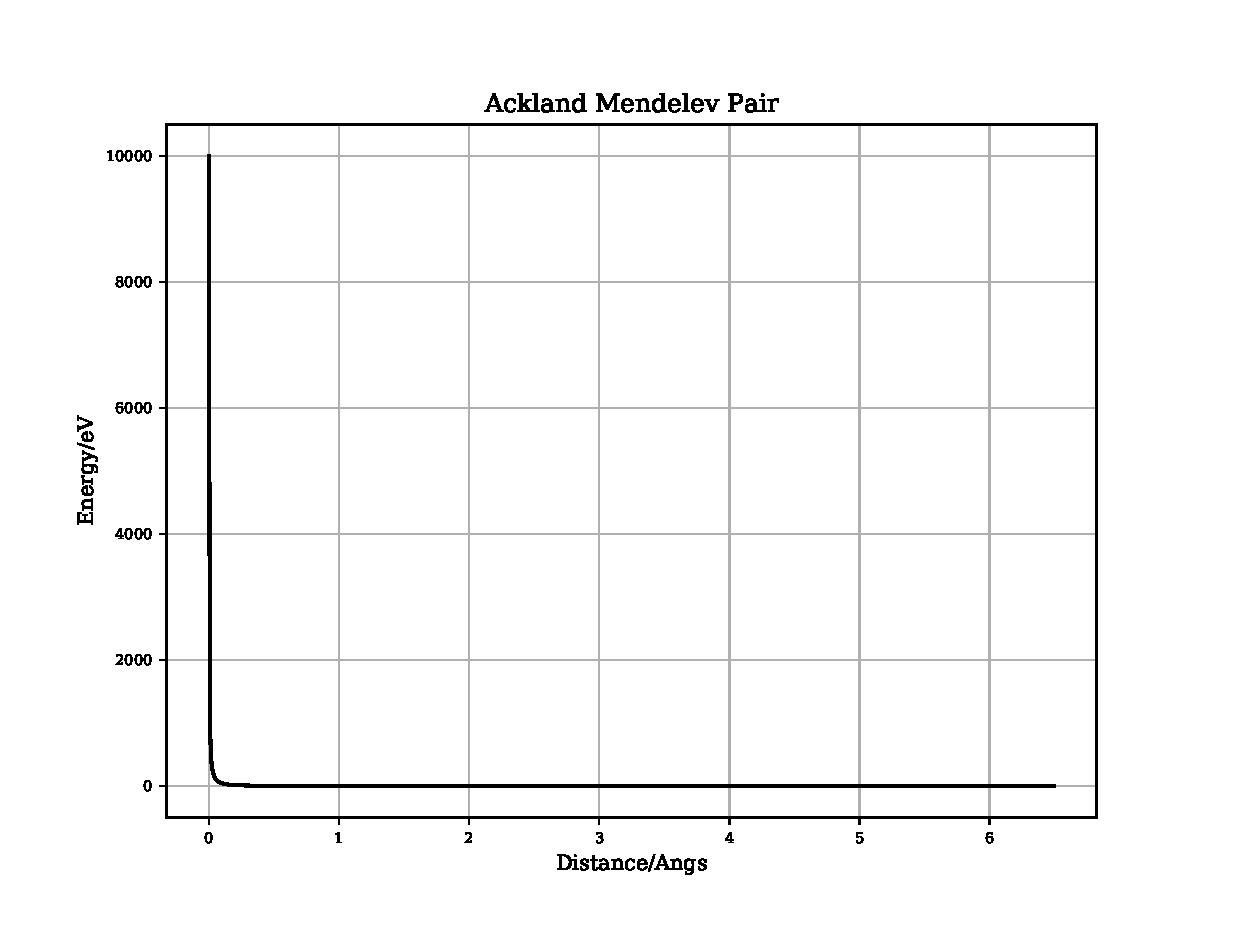
\includegraphics[scale=0.5]{appendix/functions/plots/ackland_mendelev_pair.eps}
    \caption{Ackland Mendelev Pair}
    \label{graph:graph1}
  \end{center}
\end{figure}
\FloatBarrier









%%%%%%%%%%%%%%%%%%%%%%%%%%%%%%%%%%%%%%%
% Buckingham
%%%%%%%%%%%%%%%%%%%%%%%%%%%%%%%%%%%%%%%

\subsection{Buckingham}

\begin{equation}
\begin{split}
V(r) = A \times exp(-B \times r) - \frac{C}{r^6}
\end{split}
\label{eq:eqBuckingham}
\end{equation}

\begin{lstlisting}[style=pseudocode,caption={Buckingham}]
#TYPE buckingham
#P 6.0 0.5 12.0
\end{lstlisting}

\FloatBarrier
\begin{figure}[h]
  \begin{center}
    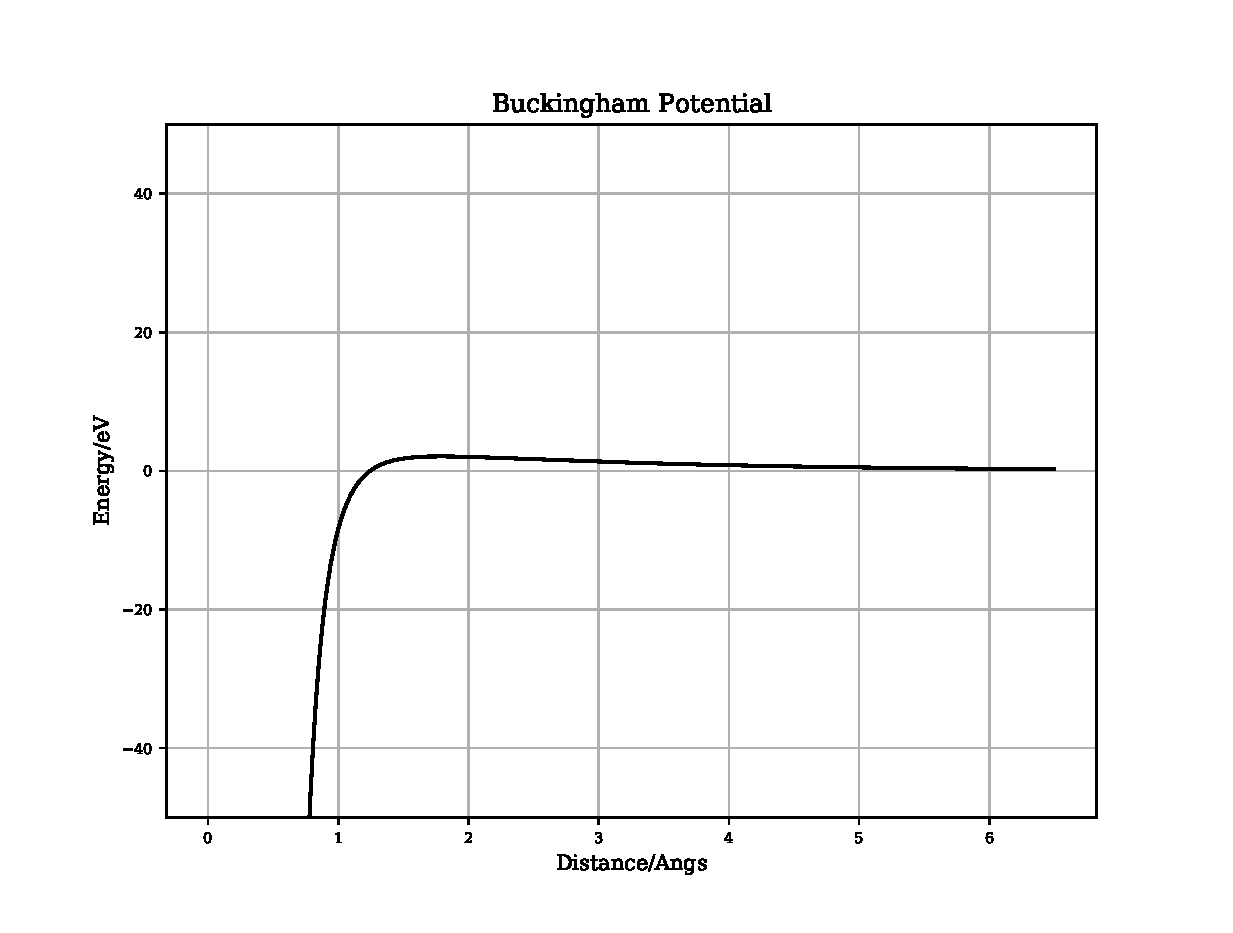
\includegraphics[scale=0.5]{appendix/functions/plots/buckingham.eps}
    \caption{Buckingham Potential}
    \label{graph:graph1}
  \end{center}
\end{figure}
\FloatBarrier






%%%%%%%%%%%%%%%%%%%%%%%%%%%%%%%%%%%%%%%
% Cubic Knot Spline
%%%%%%%%%%%%%%%%%%%%%%%%%%%%%%%%%%%%%%%

\subsection{Cubic Knot Spline}

\begin{equation}
\begin{split}
V(r) = \sum_i^N a_i (r - r_i)^3 H(r_i - r) \\
\text{where } \\
H(x) = \left\{ \begin{matrix} 0 & x<0 \\  1 & x >= 0 \end{matrix} \right . 
\end{split}
\label{eq:cubicKnotSpline}
\end{equation}


\begin{lstlisting}[style=pseudocode,caption={Cubic Knot Spline}]
#TYPE cubic_knot_spline
#P  0.0 1.0 0.02 -0.01 0.002  0.0
#PF 0.0 1.0 2.0   3.0  4.0    5.0
\end{lstlisting}

\FloatBarrier
\begin{figure}[h]
  \begin{center}
    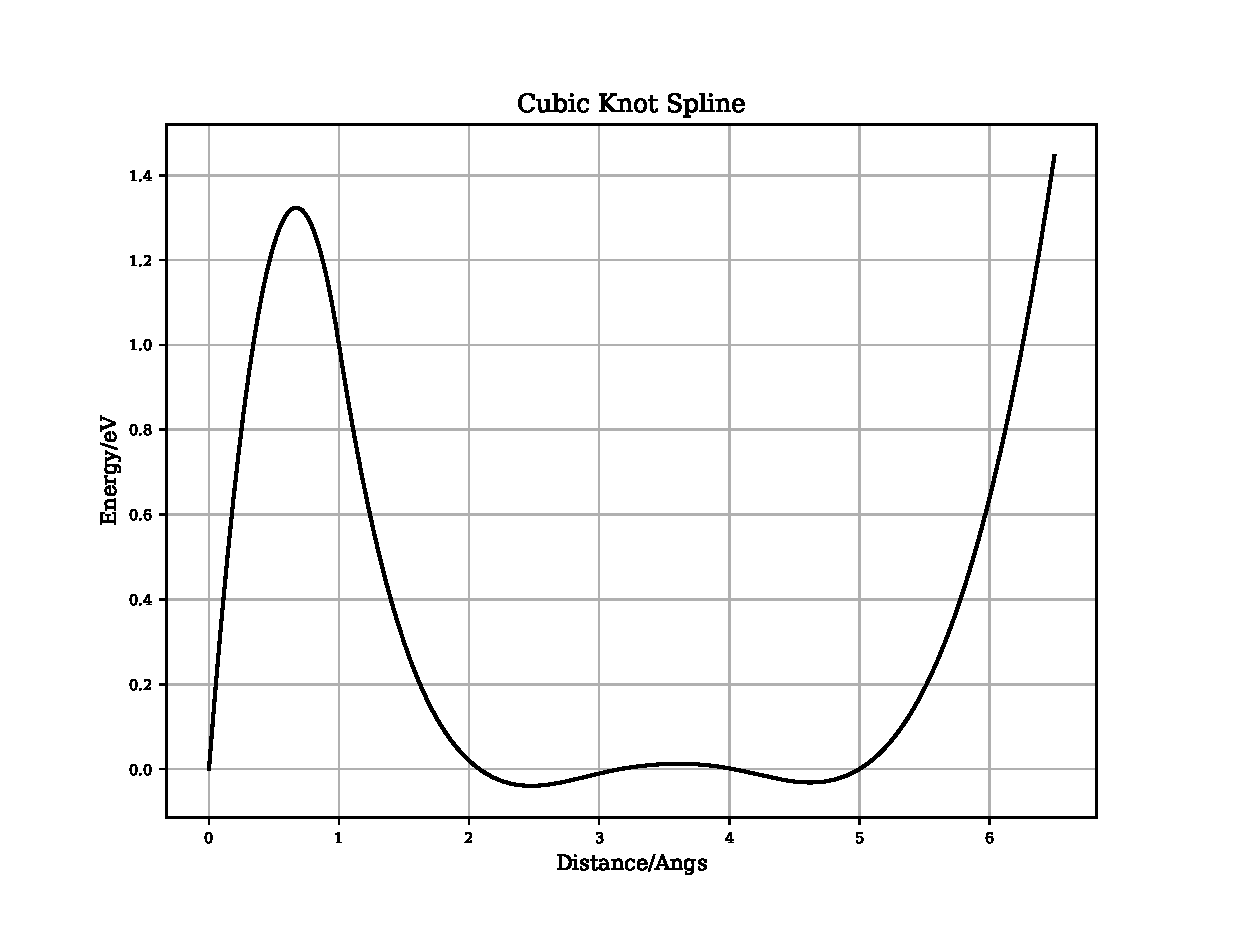
\includegraphics[scale=0.5]{appendix/functions/plots/cubic_knot_spline.eps}
    \caption{Cubic Knot Spline}
    \label{graph:graph1}
  \end{center}
\end{figure}
\FloatBarrier




%%%%%%%%%%%%%%%%%%%%%%%%%%%%%%%%%%%%%%%
% Cubic Knot Spline Fixed End
%%%%%%%%%%%%%%%%%%%%%%%%%%%%%%%%%%%%%%%

\subsection{Cubic Knot Spline Fixed End}

\begin{equation}
\begin{split}
V(r) = \sum_i^N a_i (r - r_i)^3 H(r_i - r) \\
\text{where } \\
H(x) = \left\{ \begin{matrix} 0 & x<0 \\  1 & x >= 0 \end{matrix} \right . 
\end{split}
\label{eq:cubicKnotSplineFixedEnd}
\end{equation}


\begin{lstlisting}[style=pseudocode,caption={Cubic Knot Spline Fixed End}]
#TYPE cubic_knot_spline_fixed_end
#P  0.0 1.0 0.02 -0.01 0.002  0.0
#PF 0.0 1.0 2.0   3.0  4.0    5.0   6.5   0.0   0.0
\end{lstlisting}

\FloatBarrier
\begin{figure}[h]
  \begin{center}
    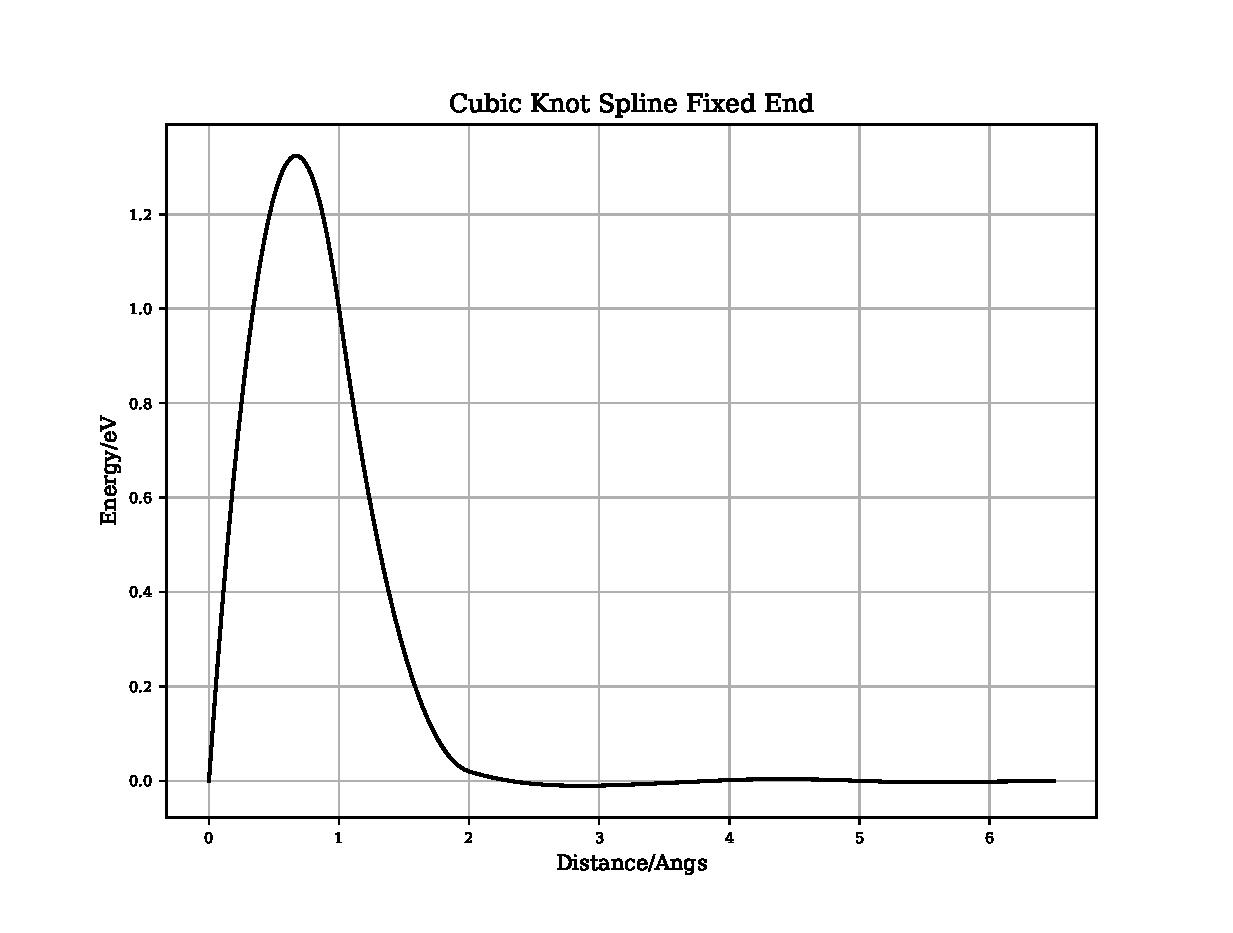
\includegraphics[scale=0.5]{appendix/functions/plots/cubic_knot_spline_fixed_end.eps}
    \caption{Cubic Knot Spline Fixed End}
    \label{graph:graph1}
  \end{center}
\end{figure}
\FloatBarrier






%%%%%%%%%%%%%%%%%%%%%%%%%%%%%%%%%%%%%%%
% Cubic Knot Spline Fixed End Pair
%%%%%%%%%%%%%%%%%%%%%%%%%%%%%%%%%%%%%%%

\subsection{Cubic Knot Spline Fixed End Pair}

\begin{equation}
\begin{split}
V(r) = \sum_i^N a_i (r - r_i)^3 H(r_i - r) \\
\text{where } \\
H(x) = \left\{ \begin{matrix} 0 & x<0 \\  1 & x >= 0 \end{matrix} \right . 
\end{split}
\label{eq:cubicKnotSplineFixedEndPair}
\end{equation}

\begin{lstlisting}[style=pseudocode,caption={Cubic Knot Spline Fixed End Pair}]
#TYPE cubic_knot_spline_fixed_end_pair
#P   0.5  0.007 -0.3  0.000001 0.002  0.0
#PF  2.0  2.5    3.0  3.5      4.0    5.0   26.0  26.0  1.0  6.5   0.0   0.0
\end{lstlisting}

\FloatBarrier
\begin{figure}[h]
  \begin{center}
    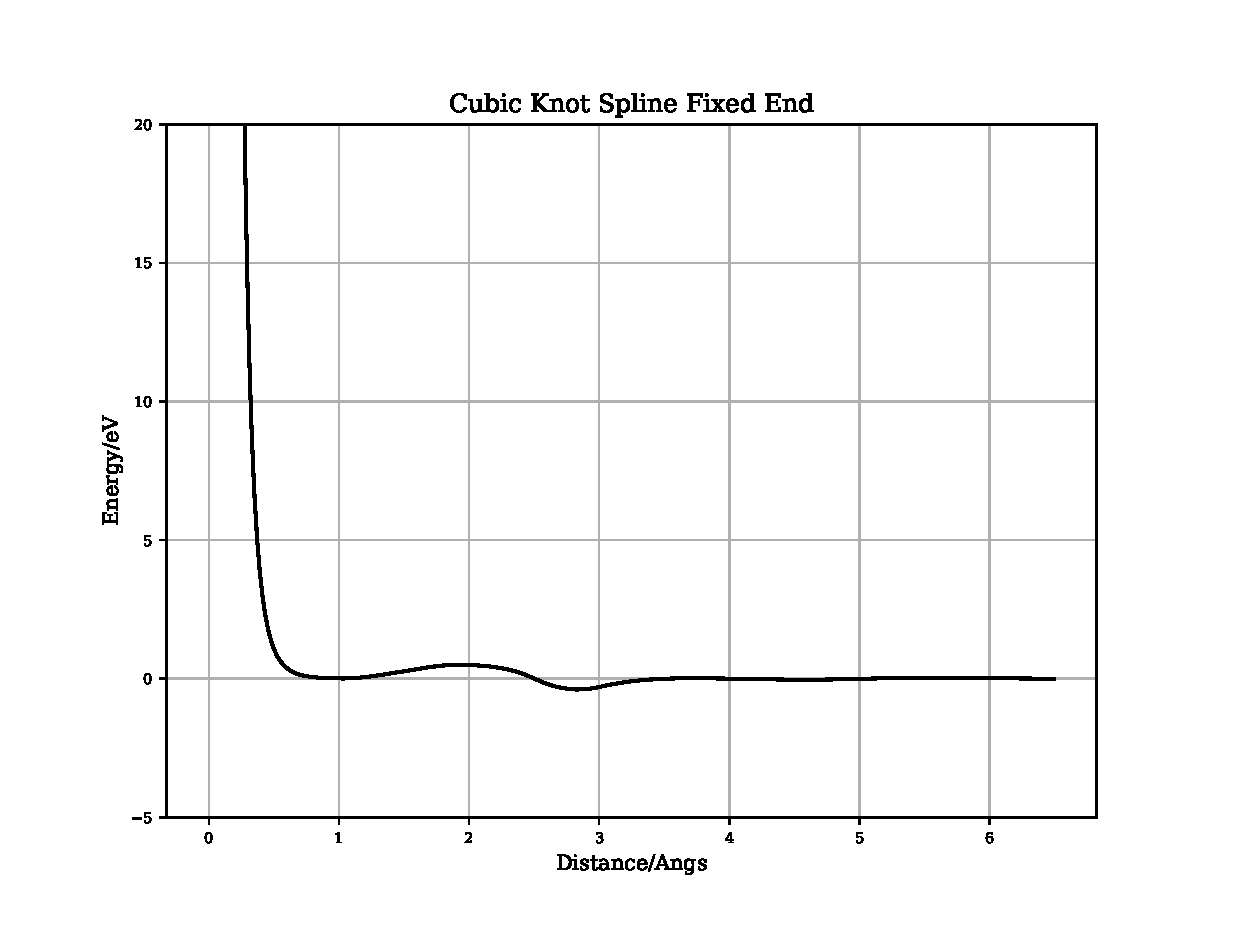
\includegraphics[scale=0.5]{appendix/functions/plots/cubic_knot_spline_fixed_end_pair.eps}
    \caption{Cubic Knot Spline Fixed End Pair}
    \label{graph:graph1}
  \end{center}
\end{figure}
\FloatBarrier





%%%%%%%%%%%%%%%%%%%%%%%%%%%%%%%%%%%%%%%
% Cubic Splines
%%%%%%%%%%%%%%%%%%%%%%%%%%%%%%%%%%%%%%%

\subsection{Cubic Splines}

\begin{equation}
\begin{split}
V(r) = \sum_i^N a_i (r - r_i)^3 H(r_i - r) \\
\text{where } \\
H(x) = \left\{ \begin{matrix} 0 & x<0 \\  1 & x >= 0 \end{matrix} \right . 
\end{split}
\label{eq:cubicSpline}
\end{equation}

This function requires two sets of parameters.  P is a list of N coefficients and PF is a list of N cutoffs.  The cubic polynomials are summed and individually scaled by the coefficients, and by virtue of its form and the heaviside step function, they cut off at the desired radius. 

\begin{lstlisting}[style=pseudocode,caption={Cubic Splines}]
#TYPE cubic_spline
#P -165.0 -78.5 -78.15 1.868
#PF 0.976 1.15 1.216 1.650
\end{lstlisting}

\FloatBarrier
\begin{figure}[h]
  \begin{center}
    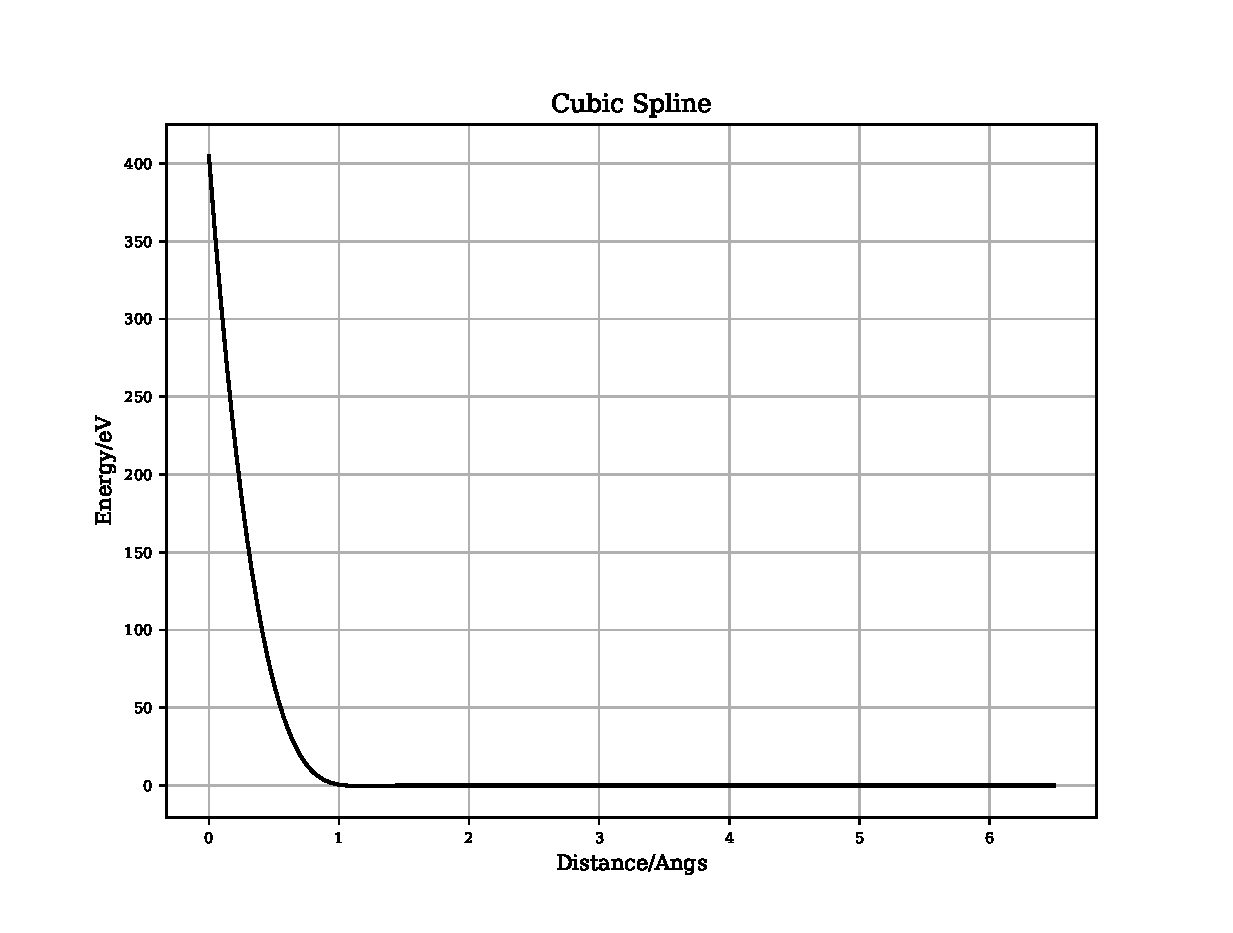
\includegraphics[scale=0.5]{appendix/functions/plots/cubic_spline.eps}
    \caption{Ackland Embedding}
    \label{graph:graph1}
  \end{center}
\end{figure}
\FloatBarrier


\subsection{Cubic Spline Plus ZBL}

\begin{equation}
\begin{split}
V(r) = \left\{ \begin{matrix} z(r) & r <r_1 \\  a_0 + a_1 r + a_2 r^2 + a_3 r^3 & r_1 <= r <= r_2  \\   \sum_i^N a_i (r - r_i)^3 H(r_i - r) & r > r_2 \end{matrix} \right . 
\text{where } \\
H(x) = \left\{ \begin{matrix} 0 & x<0 \\  1 & x >= 0 \end{matrix} \right . 
\end{split}
\label{eq:cubicSplineZBL}
\end{equation}

This function requires two sets of parameters.  P is a list of N coefficients and PF is a list of N cutoffs.  The cubic polynomials are summed and individually scaled by the coefficients, and by virtue of its form and the heaviside step function, they cut off at the desired radius. 

\begin{lstlisting}[style=pseudocode,caption={Cubic Splines Plus ZBL}]
#TYPE cubic_spline_zbl
#P 0.707937643181 1.00089008639 0.978759224081 -0.0460365116314 -0.00762125172653 -0.0209035950064 0.00938859724754 0.000854708875904 0.0230647235533 0.011459696349 0.023419434017 0.0220932107774 0.0325043051929 -0.0425828941427 -0.0147289840464 0.0138435254515 0.000880298224106 -0.0134658842396 0.00102524605929 
#PF 1.7 1.8 2.0 2.1 2.2 2.3 2.4 2.5 2.6 2.7 2.8 3.0 3.3 3.7 4.2 4.7 5.3 6.0 6.5 26.0 26.0 0.55 1.7 1.0 
\end{lstlisting}

\FloatBarrier
\begin{figure}[h]
  \begin{center}
    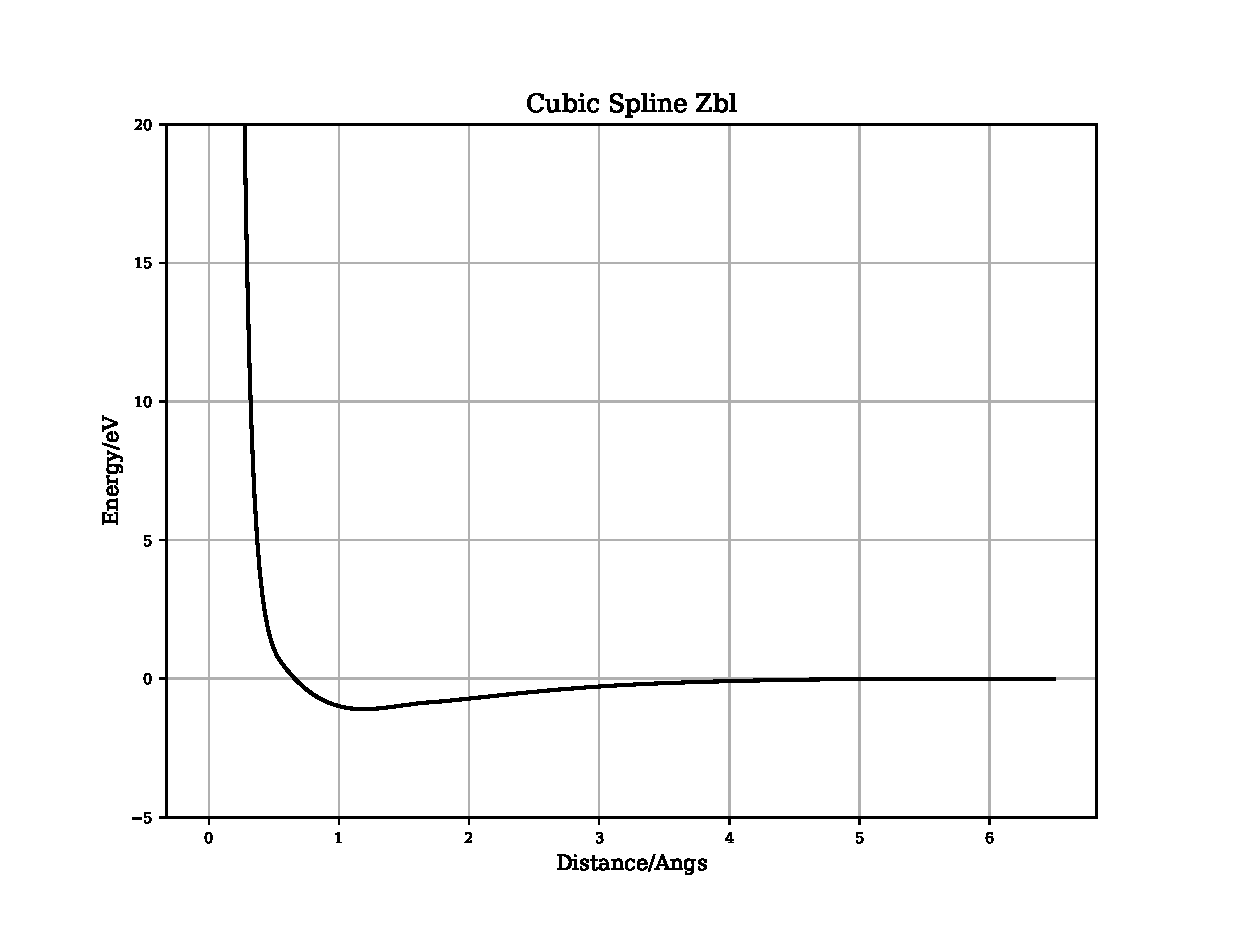
\includegraphics[scale=0.5]{appendix/functions/plots/cubic_spline_zbl.eps}
    \caption{Ackland Embedding}
    \label{graph:graph1}
  \end{center}
\end{figure}
\FloatBarrier


\begin{lstlisting}[style=pseudocode,caption={Cubic Splines Plus ZBL}]
#TYPE cubic_spline_zbl
#P 1.00048374974 0.999953842306 0.817335736705 -0.0469506463728 -0.118042905174 0.00429308591859 0.024332744974 0.0454260983505 0.0205392979832 0.415064378029 0.649740384042 0.0433627017609 0.047890256076 0.026097144285 0.0106186840232 0.0138597059993 -0.0172453611171 -0.00144350314717 -0.00170969310596 
#PF 1.7 1.8 2.0 2.1 2.2 2.3 2.4 2.5 2.6 2.7 2.8 3.0 3.3 3.7 4.2 4.7 5.3 6.0 6.5 26.0 26.0 0.6 1.6 1.0  
\end{lstlisting}

\FloatBarrier
\begin{figure}[h]
  \begin{center}
    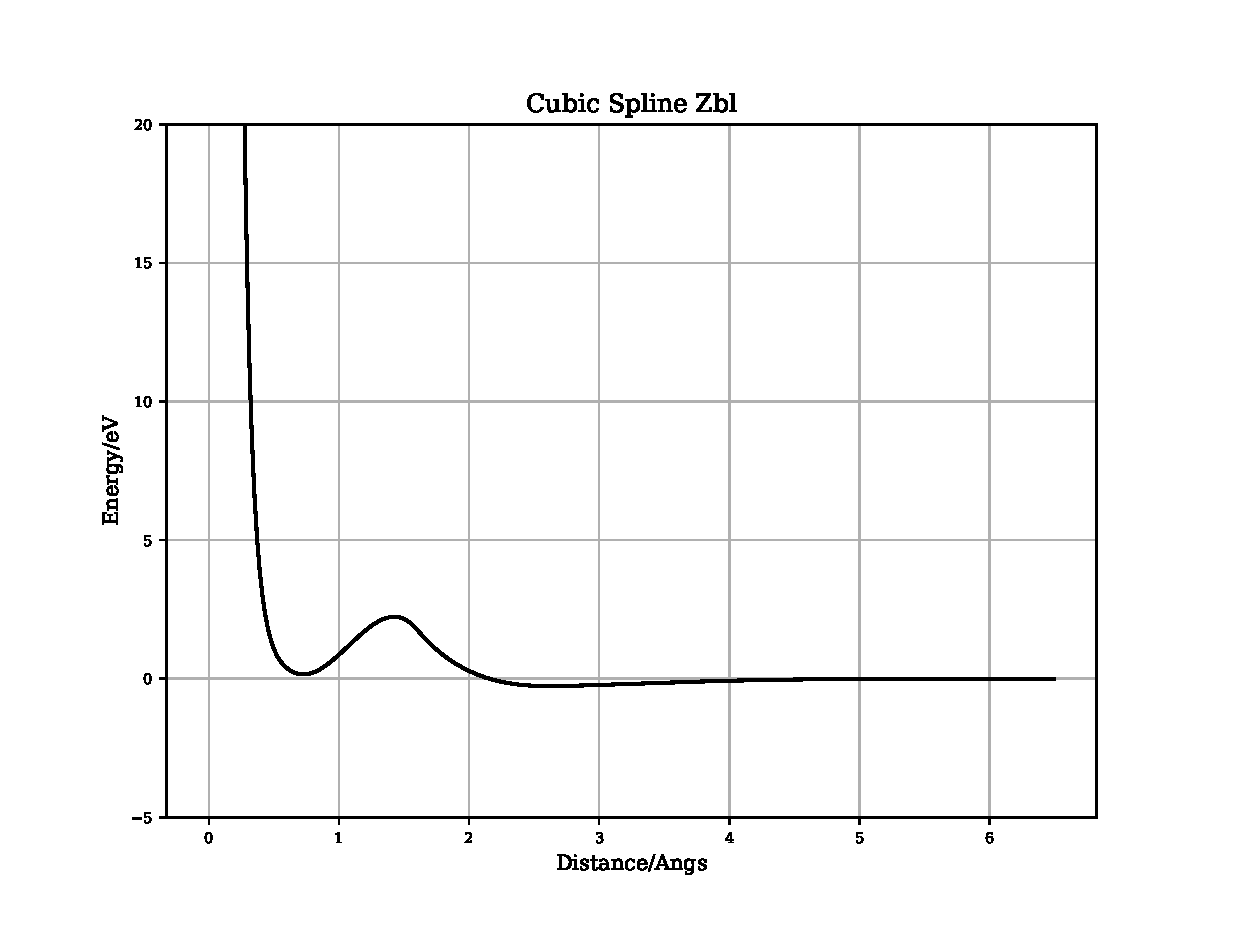
\includegraphics[scale=0.5]{appendix/functions/plots/cubic_spline_zbl_2.eps}
    \caption{Ackland Embedding}
    \label{graph:graph1}
  \end{center}
\end{figure}
\FloatBarrier



%%%%%%%%%%%%%%%%%%%%%%%%%%%%%%%%%%%%%%%
% Embedding A
%%%%%%%%%%%%%%%%%%%%%%%%%%%%%%%%%%%%%%%

\subsection{Embedding A - Finnis Sinclair}

\begin{equation}
\begin{split}
F(\rho) = -a \sqrt{\rho}
\end{split}
\label{eq:finnisSinclair}
\end{equation}

This function requires one parameter\cite{finnissinclair}.

\begin{lstlisting}[style=pseudocode,caption={Embedding A}]
#TYPE embedding_a
#P 0.1
\end{lstlisting}

\FloatBarrier
\begin{figure}[h]
  \begin{center}
    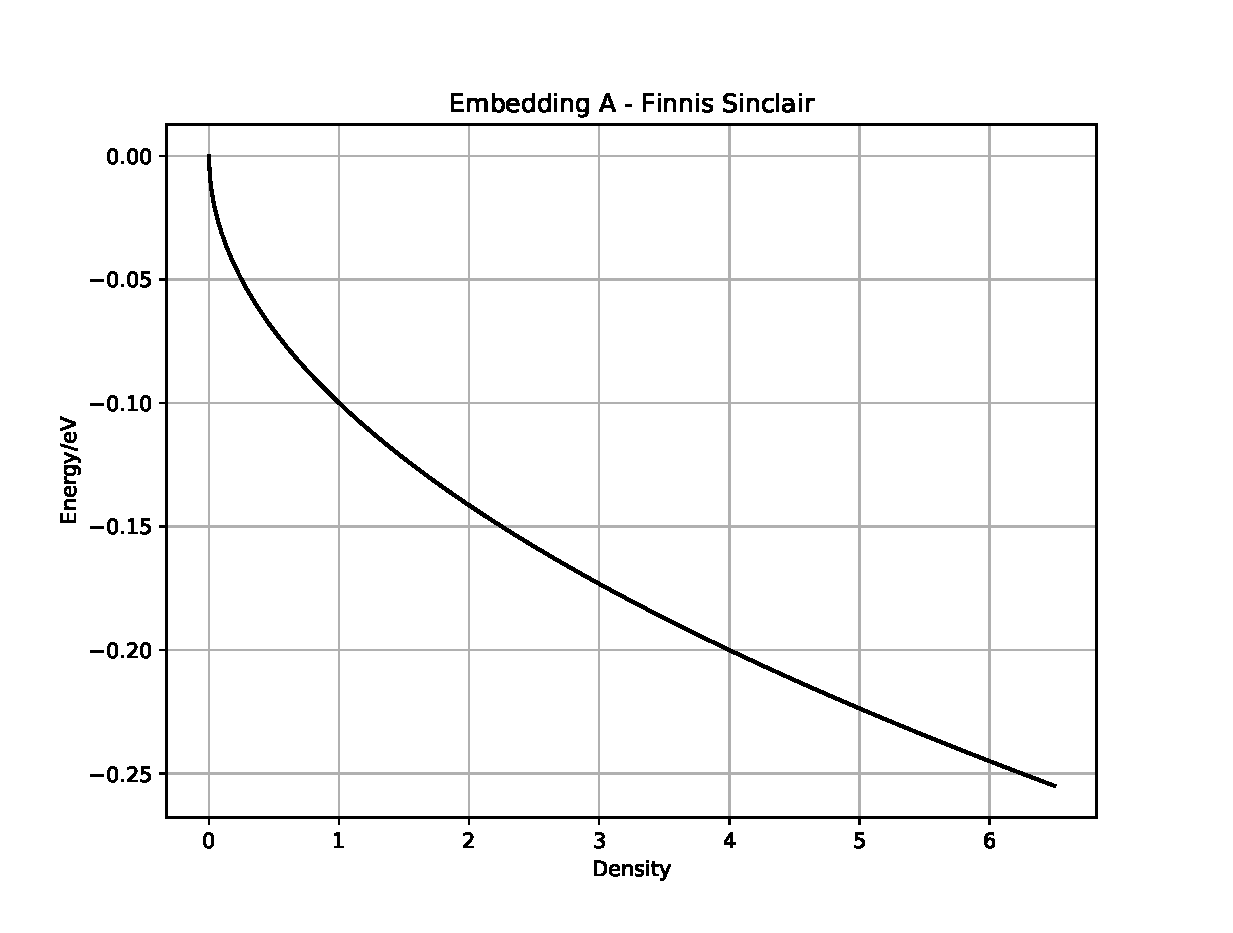
\includegraphics[scale=0.5]{appendix/functions/plots/embedding_a.eps}
    \caption{Embedding A}
    \label{graph:graph1}
  \end{center}
\end{figure}
\FloatBarrier







%%%%%%%%%%%%%%%%%%%%%%%%%%%%%%%%%%%%%%%
% Embedding B
%%%%%%%%%%%%%%%%%%%%%%%%%%%%%%%%%%%%%%%

\subsection{Embedding B - Mendelev}

\begin{equation}
\begin{split}
F(\rho) = -\sqrt{\rho} + a \rho^2
\end{split}
\label{eq:mendelevEmbedding}
\end{equation}

This function requires one parameter. 
Development of new interatomic potentials appropriate for crystalline and liquid iron, 2003.

\begin{lstlisting}[style=pseudocode,caption={Embedding B}]
#TYPE embedding_b
#P 0.1
\end{lstlisting}

\FloatBarrier
\begin{figure}[h]
  \begin{center}
    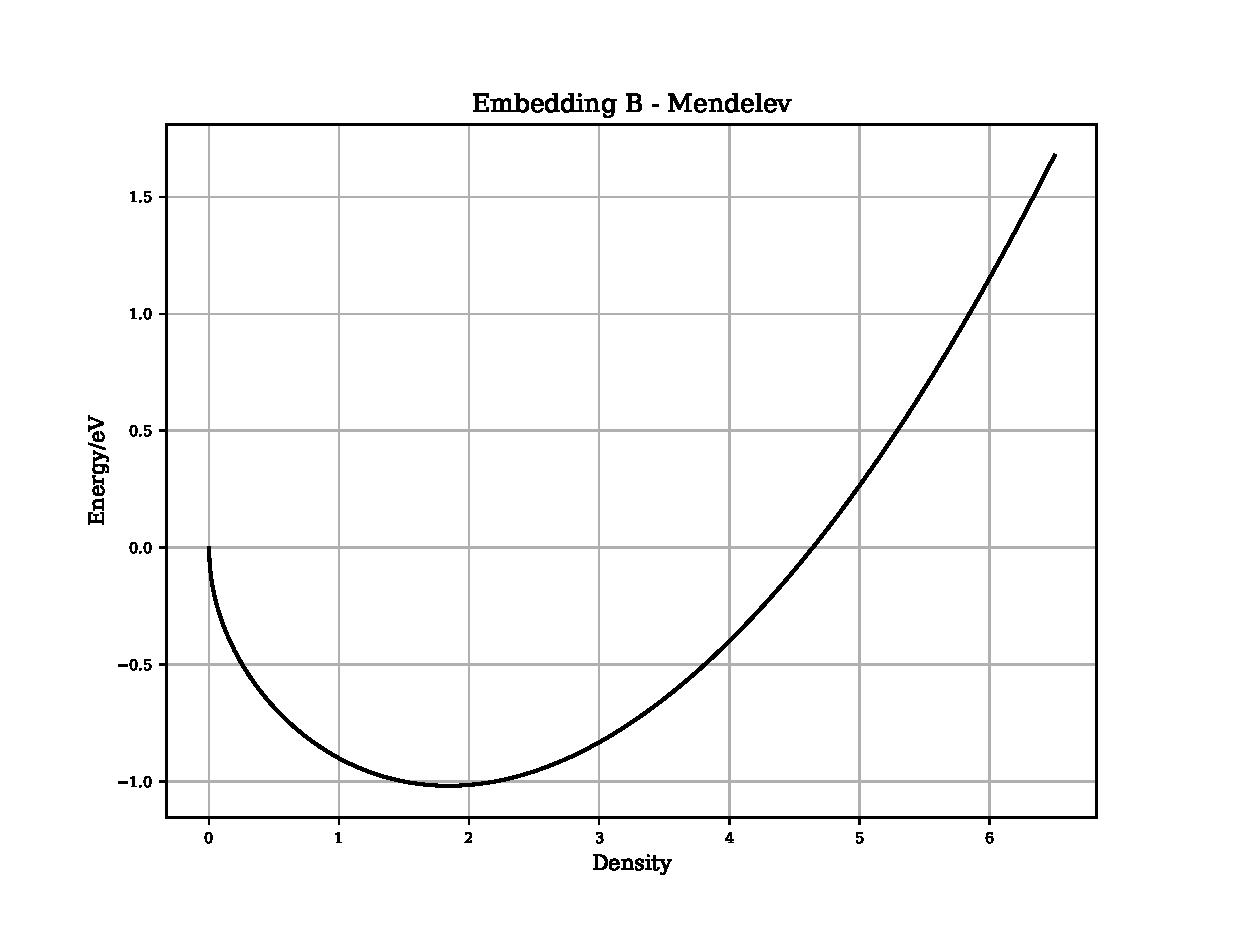
\includegraphics[scale=0.5]{appendix/functions/plots/embedding_b.eps}
    \caption{Embedding B}
    \label{graph:graph1}
  \end{center}
\end{figure}
\FloatBarrier








%%%%%%%%%%%%%%%%%%%%%%%%%%%%%%%%%%%%%%%
% Embedding C
%%%%%%%%%%%%%%%%%%%%%%%%%%%%%%%%%%%%%%%

\subsection{Embedding C}

\begin{equation}
\begin{split}
F(\rho) = a \sqrt{\rho} + b \rho^2
\end{split}
\label{eq:embeddingC}
\end{equation}


\begin{lstlisting}[style=pseudocode,caption={Embedding C}]
#TYPE embedding_c
#P 0.1 0.1
\end{lstlisting}

\FloatBarrier
\begin{figure}[h]
  \begin{center}
    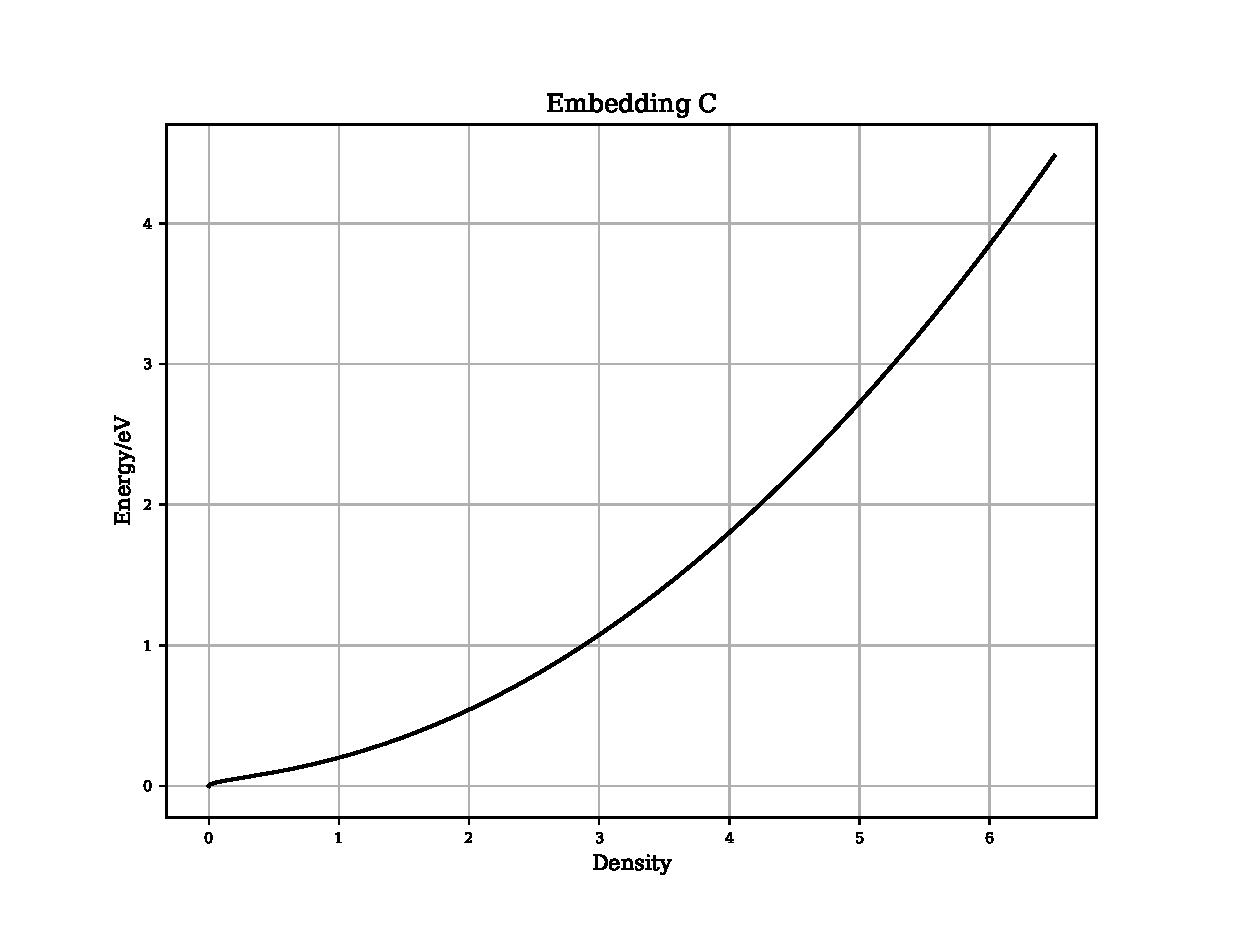
\includegraphics[scale=0.5]{appendix/functions/plots/embedding_c.eps}
    \caption{Embedding C}
    \label{graph:graph1}
  \end{center}
\end{figure}
\FloatBarrier







%%%%%%%%%%%%%%%%%%%%%%%%%%%%%%%%%%%%%%%
% Embedding D
%%%%%%%%%%%%%%%%%%%%%%%%%%%%%%%%%%%%%%%

\subsection{Embedding D - Ackland-Mendelev}

\begin{equation}
\begin{split}
F(\rho) = -\sqrt({\rho} + a \rho^2 + b \rho^4
\end{split}
\label{eq:embeddingD}
\end{equation}

This function requires one parameter. 
Development of an interatomic potential for phosphorus impurities in α-iron, 2004.


\begin{lstlisting}[style=pseudocode,caption={Embedding D}]
#TYPE embedding_d
#P 0.05 -0.00001
\end{lstlisting}

\FloatBarrier
\begin{figure}[h]
  \begin{center}
    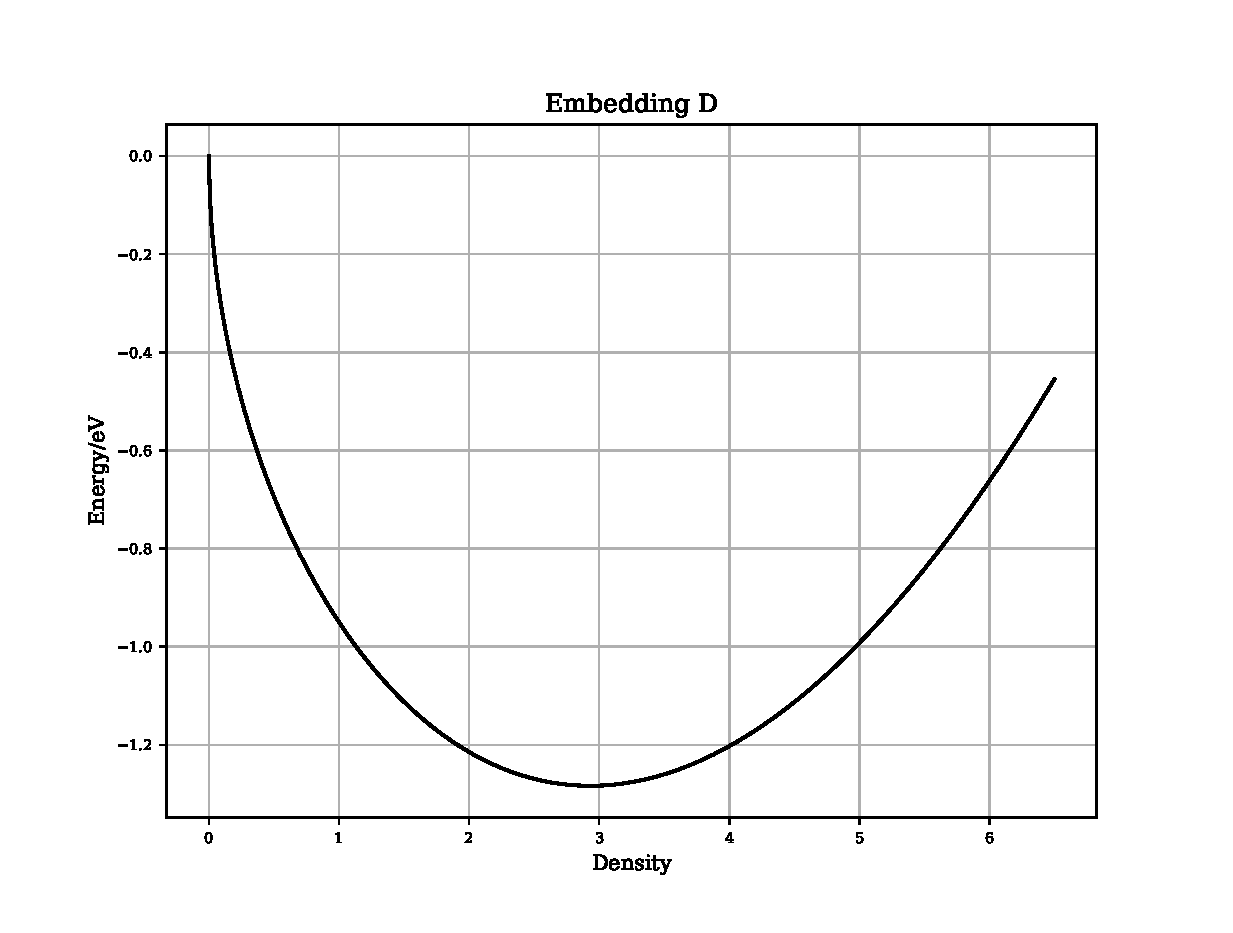
\includegraphics[scale=0.5]{appendix/functions/plots/embedding_d.eps}
    \caption{Embedding D}
    \label{graph:graph1}
  \end{center}
\end{figure}
\FloatBarrier







%%%%%%%%%%%%%%%%%%%%%%%%%%%%%%%%%%%%%%%
% Embedding E
%%%%%%%%%%%%%%%%%%%%%%%%%%%%%%%%%%%%%%%

\subsection{Embedding E}

\begin{equation}
\begin{split}
F(\rho) = a \sqrt{\rho} + b \rho^2 + c \rho^4
\end{split}
\label{eq:embeddingE}
\end{equation}

\begin{lstlisting}[style=pseudocode,caption={Embedding E}]
#TYPE embedding_e
#P -0.8 0.05 -0.00001
\end{lstlisting}

\FloatBarrier
\begin{figure}[h]
  \begin{center}
    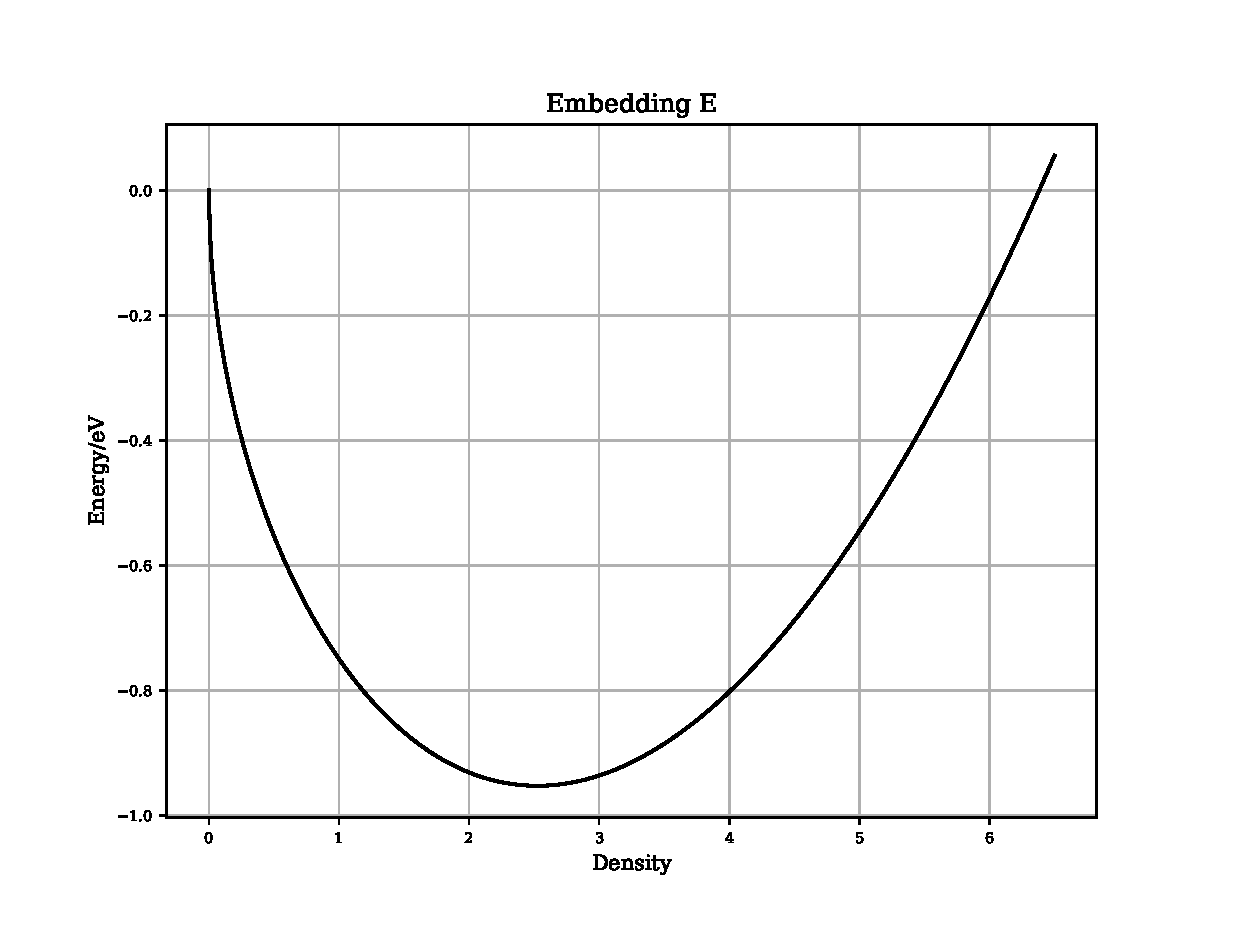
\includegraphics[scale=0.5]{appendix/functions/plots/embedding_e.eps}
    \caption{Ackland Embedding}
    \label{graph:graph1}
  \end{center}
\end{figure}
\FloatBarrier




%%%%%%%%%%%%%%%%%%%%%%%%%%%%%%%%%%%%%%%
% Embedding F
%%%%%%%%%%%%%%%%%%%%%%%%%%%%%%%%%%%%%%%

\subsection{Embedding F}

\begin{equation}
\begin{split}
F(\rho) = a \sqrt{\rho} + b \rho^2 + \rho^4
\end{split}
\label{eq:embeddingF}
\end{equation}

\begin{lstlisting}[style=pseudocode,caption={Embedding F}]
#TYPE embedding_f
#P -0.8 0.05
\end{lstlisting}

\FloatBarrier
\begin{figure}[h]
  \begin{center}
    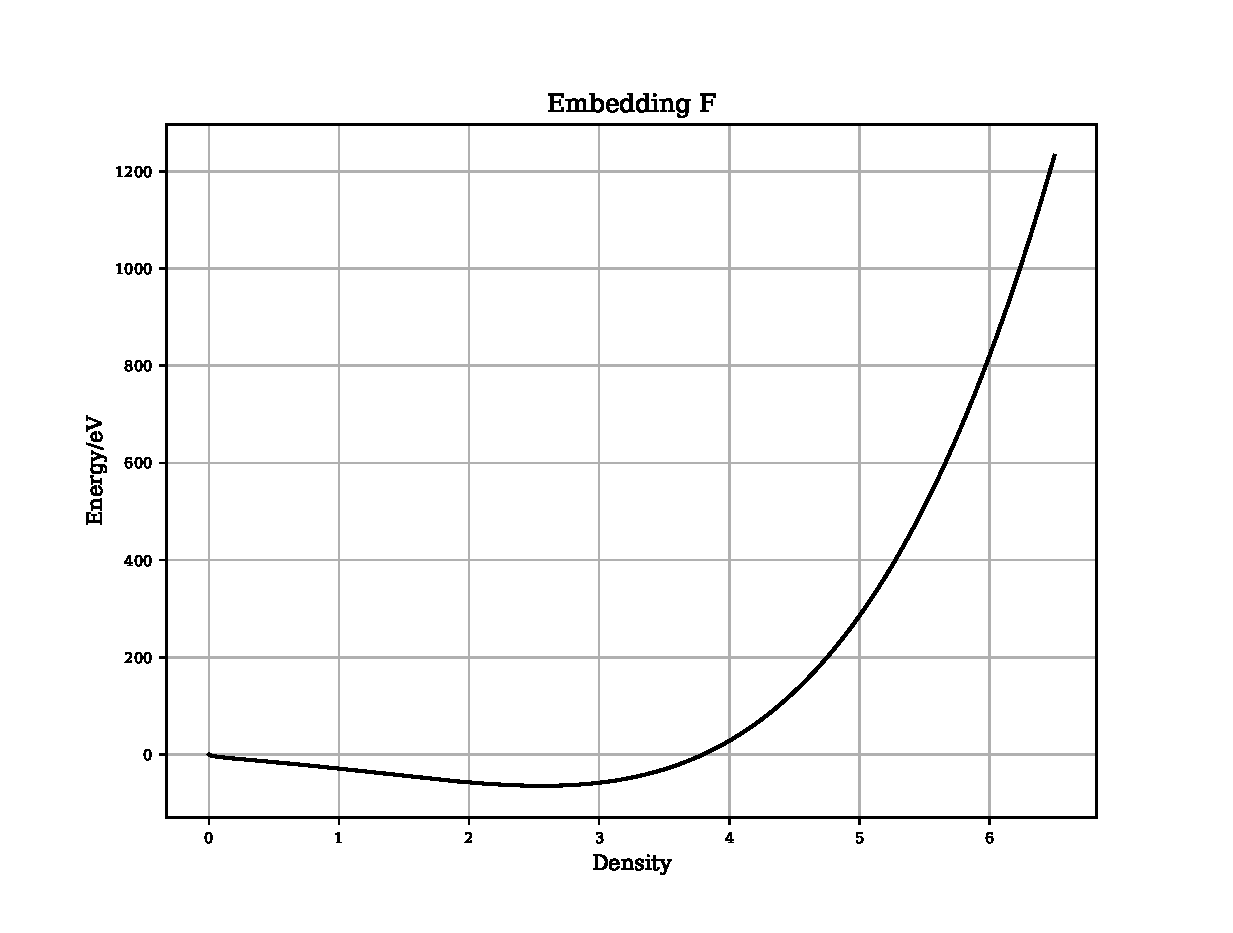
\includegraphics[scale=0.5]{appendix/functions/plots/embedding_f.eps}
    \caption{Embedding F Function Plot}
    \label{graph:embeddingFPlot}
  \end{center}
\end{figure}

\FloatBarrier




%%%%%%%%%%%%%%%%%%%%%%%%%%%%%%%%%%%%%%%
% Embedding G
%%%%%%%%%%%%%%%%%%%%%%%%%%%%%%%%%%%%%%%

\subsection{Embedding G}

\begin{equation}
\begin{split}
F(\rho) = a \sqrt{\rho} + b \rho^2 + f \rho^4
\end{split}
\label{eq:embeddingG}
\end{equation}

\begin{lstlisting}[style=pseudocode,caption={Embedding F}]
#TYPE embedding_g
#P -9.15 5.57
#PF 0.01
\end{lstlisting}

\FloatBarrier
\begin{figure}[h]
  \begin{center}
    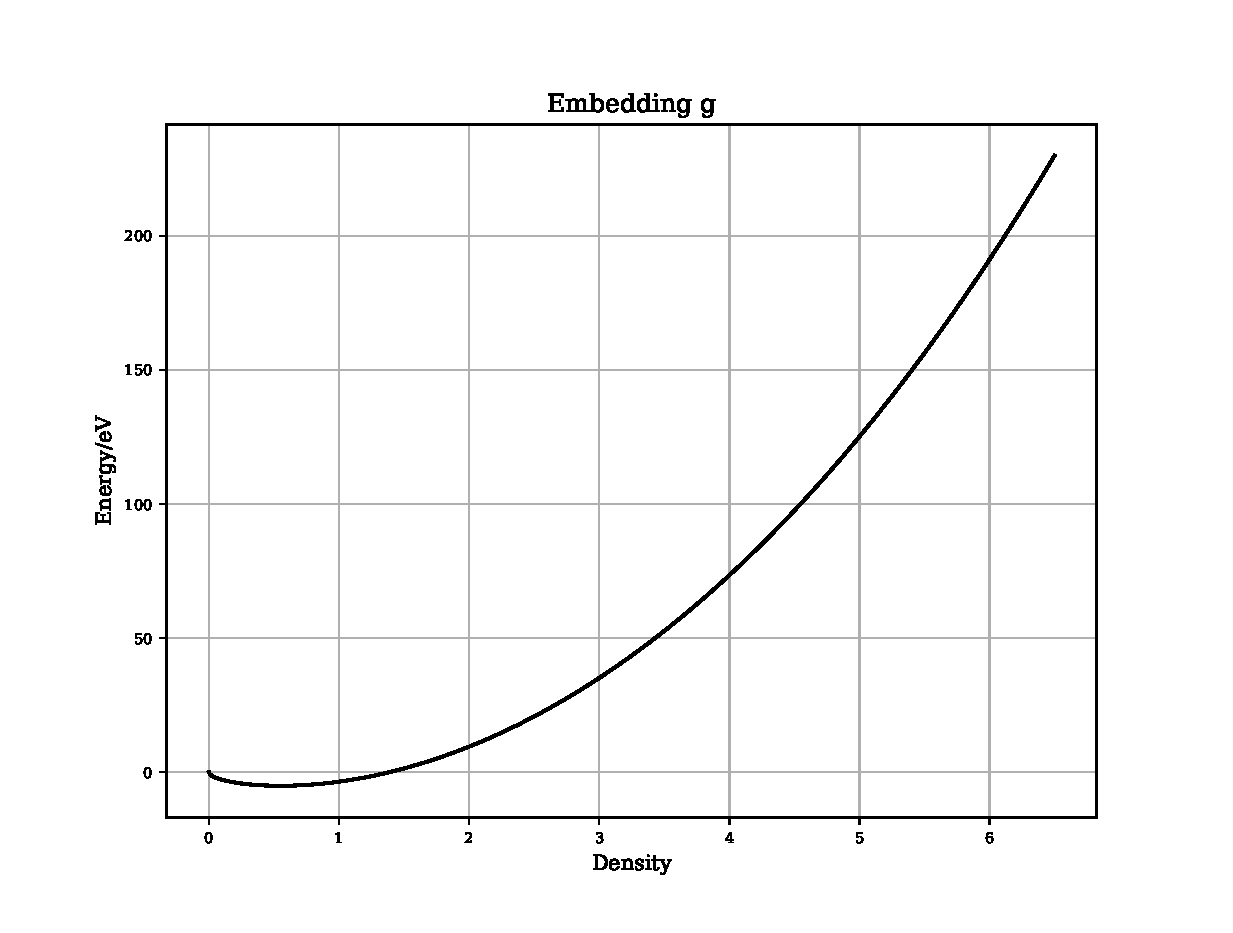
\includegraphics[scale=0.5]{appendix/functions/plots/embedding_g.eps}
    \caption{Embedding G Function Plot}
    \label{graph:embeddingGPlot}
  \end{center}
\end{figure}

\FloatBarrier




\FloatBarrier








%%%%%%%%%%%%%%%%%%%%%%%%%%%%%%%%%%%%%%%
% Lennard-Jones
%%%%%%%%%%%%%%%%%%%%%%%%%%%%%%%%%%%%%%%

\subsection{Lennard-Jones}

\begin{equation}
\begin{split}
V(r) = e \left(\left(\frac{r_m}{r}\right)^{12} - 2 \left(\frac{r_m}{r}\right)^6\right)
\end{split}
\label{eq:eqLennardJones}
\end{equation}

\begin{lstlisting}[style=pseudocode,caption={Lennard-Jones}]
#TYPE lennard_jones
#P 2.3 3.5
\end{lstlisting}

\FloatBarrier
\begin{figure}[h]
  \begin{center}
    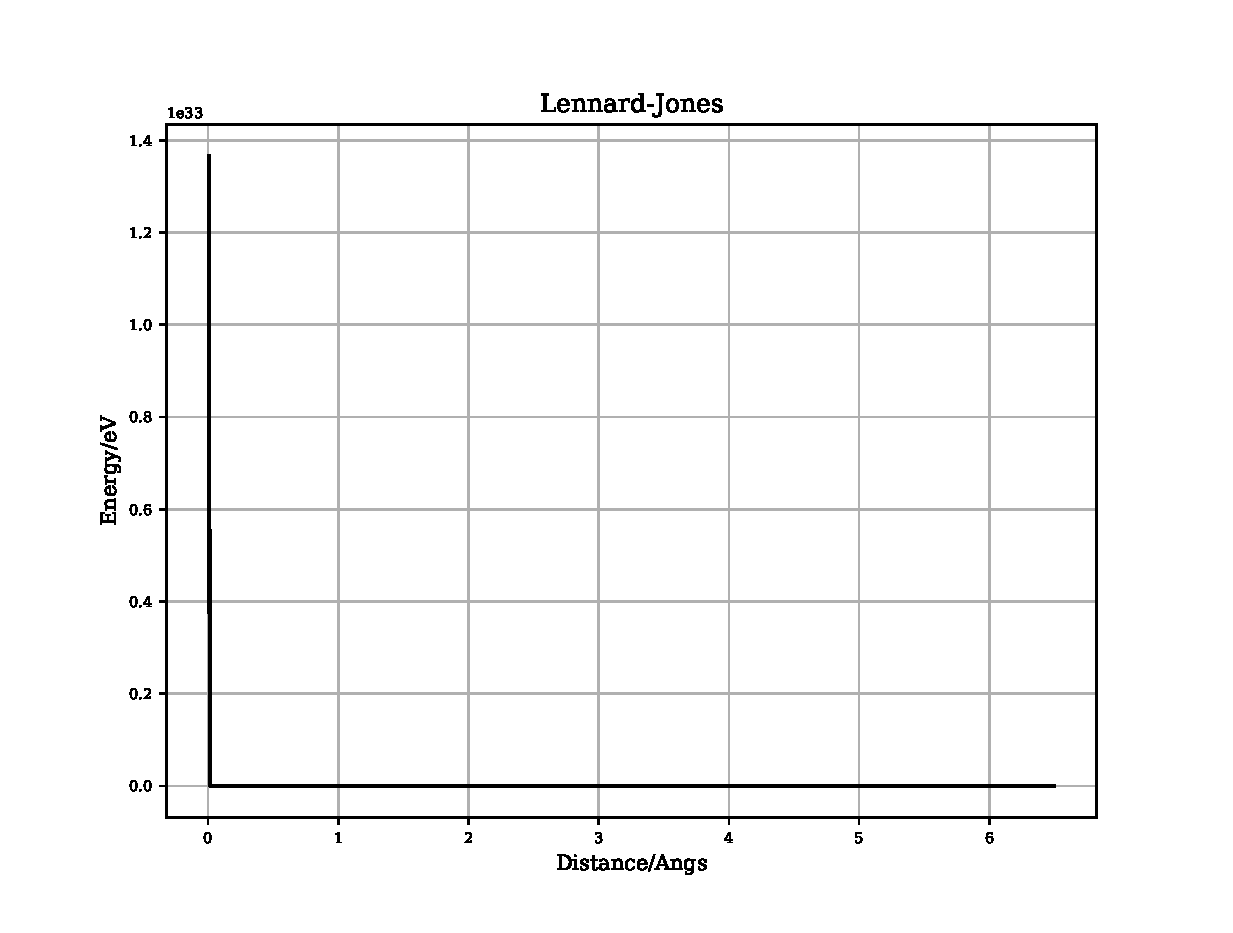
\includegraphics[scale=0.5]{appendix/functions/plots/lennard_jones.eps}
    \caption{Lennard-Jones}
    \label{graph:Lennard-Jones}
  \end{center}
\end{figure}
\FloatBarrier







%%%%%%%%%%%%%%%%%%%%%%%%%%%%%%%%%%%%%%%
% Morse
%%%%%%%%%%%%%%%%%%%%%%%%%%%%%%%%%%%%%%%

\subsection{Morse}

\begin{equation}
\begin{split}
V(r) = exp(-2 a (r - r_e)) - 2 exp (-a \times (r - r_e))
\end{split}
\label{eq:eqMorse}
\end{equation}

\begin{lstlisting}[style=pseudocode,caption={Morse}]
#TYPE morse
#P 4.669 1.256 2.8
\end{lstlisting}

\FloatBarrier
\begin{figure}[h]
  \begin{center}
    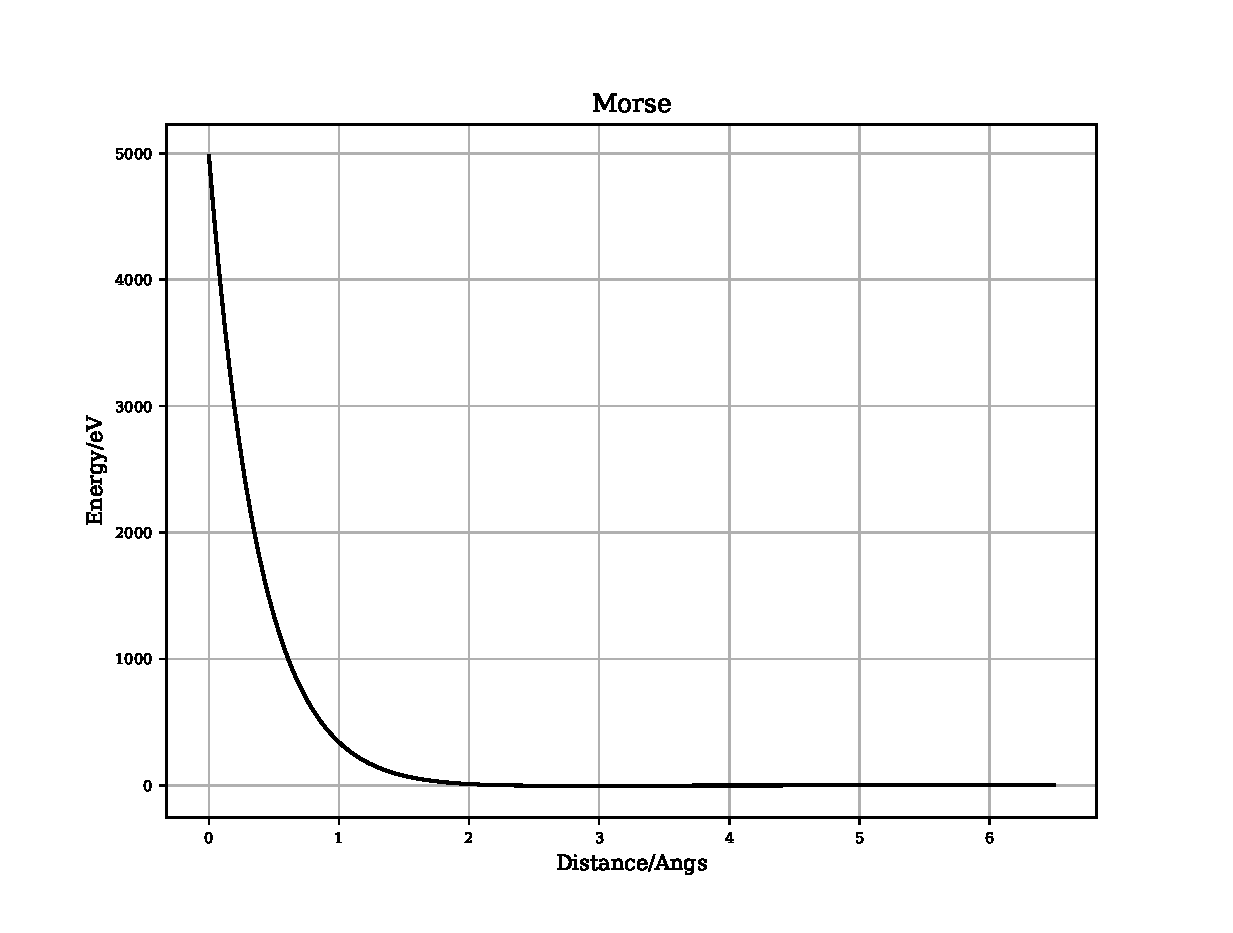
\includegraphics[scale=0.5]{appendix/functions/plots/morse.eps}
    \caption{Morse}
    \label{graph:graph1}
  \end{center}
\end{figure}
\FloatBarrier






%%%%%%%%%%%%%%%%%%%%%%%%%%%%%%%%%%%%%%%
% Slater 4S (Squared)
%%%%%%%%%%%%%%%%%%%%%%%%%%%%%%%%%%%%%%%

\subsection{Slater 4S (Squared)}

\begin{equation}
\begin{split}
\rho(r) = (N_s r^3 exp(-\eta r))^2 
\end{split}
\label{eq:slater4S}
\end{equation}

\begin{lstlisting}[style=pseudocode,caption={Slater 4S}]
#TYPE slater_4s
#P 5.0 1.323
\end{lstlisting}

\FloatBarrier
\begin{figure}[h]
  \begin{center}
    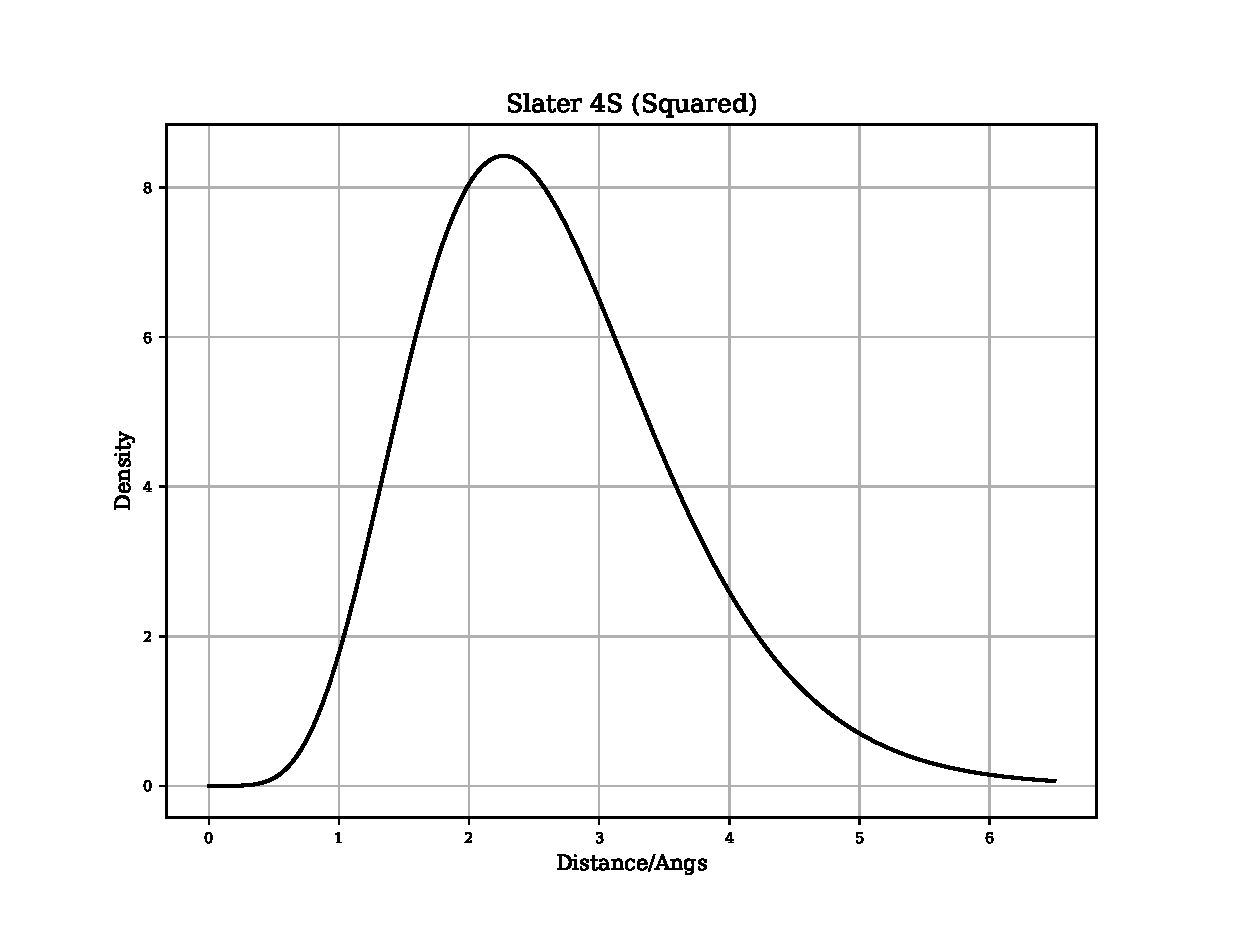
\includegraphics[scale=0.5]{appendix/functions/plots/slater_4s.eps}
    \caption{Quadratic Density}
    \label{graph:graph1}
  \end{center}
\end{figure}
\FloatBarrier






%%%%%%%%%%%%%%%%%%%%%%%%%%%%%%%%%%%%%%%
% ZBL
%%%%%%%%%%%%%%%%%%%%%%%%%%%%%%%%%%%%%%%

\subsection{ZBL}

\begin{equation}
\begin{split}
\phi(x) = 0.181 e^{-3.2x} + 0.5099 e^{-0.9423x} + 0.2802 e^{-0.4029x} + 0.02817 e^{-0.2016x} \\
\text{where } a_{ij} = \frac{0.8854 a_0}{Z^{0.23}_i + Z^{0.23}_j} \\
\text{and } a_0 = 0.529 \text{ angstrom}
\end{split}
\label{eq:ZBL}
\end{equation}

\begin{lstlisting}[style=pseudocode,caption={ZBL}]
#TYPE zbl
#P 26.0 26.0
\end{lstlisting}

\FloatBarrier
\begin{figure}[h]
  \begin{center}
    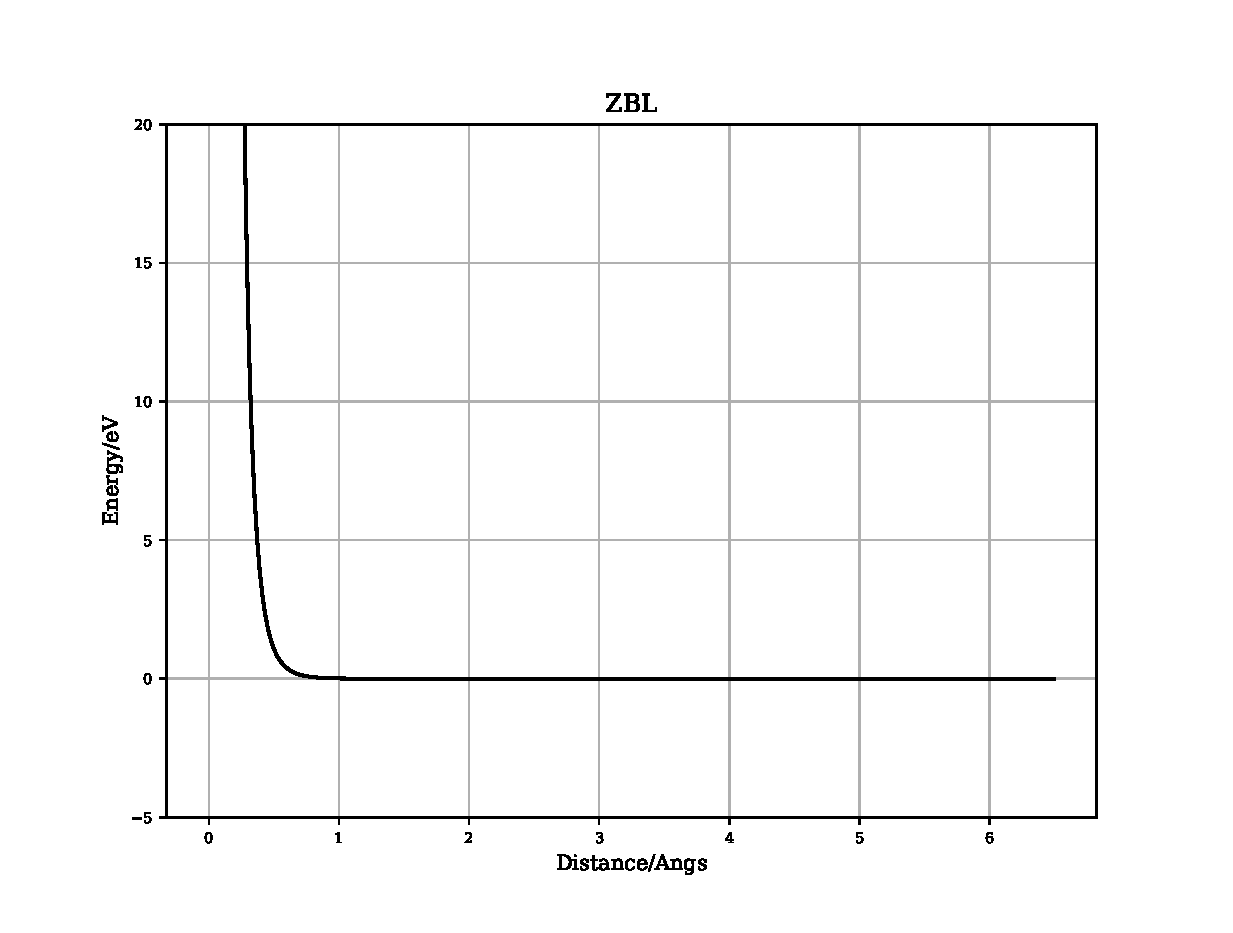
\includegraphics[scale=0.5]{appendix/functions/plots/zbl.eps}
    \caption{ZBL}
    \label{graph:graph1}
  \end{center}
\end{figure}
\FloatBarrier






%%%%%%%%%%%%%%%%%%%%%%%%%%%%%%%%%%%%%%%
% ZERO
%%%%%%%%%%%%%%%%%%%%%%%%%%%%%%%%%%%%%%%

\subsection{Zero}

\begin{equation}
\begin{split}
f(x) = 0
\end{split}
\label{eq:zero}
\end{equation}

\begin{lstlisting}[style=pseudocode,caption={Zero}]
#TYPE zero
#P 0.0
\end{lstlisting}

\FloatBarrier
\begin{figure}[h]
  \begin{center}
    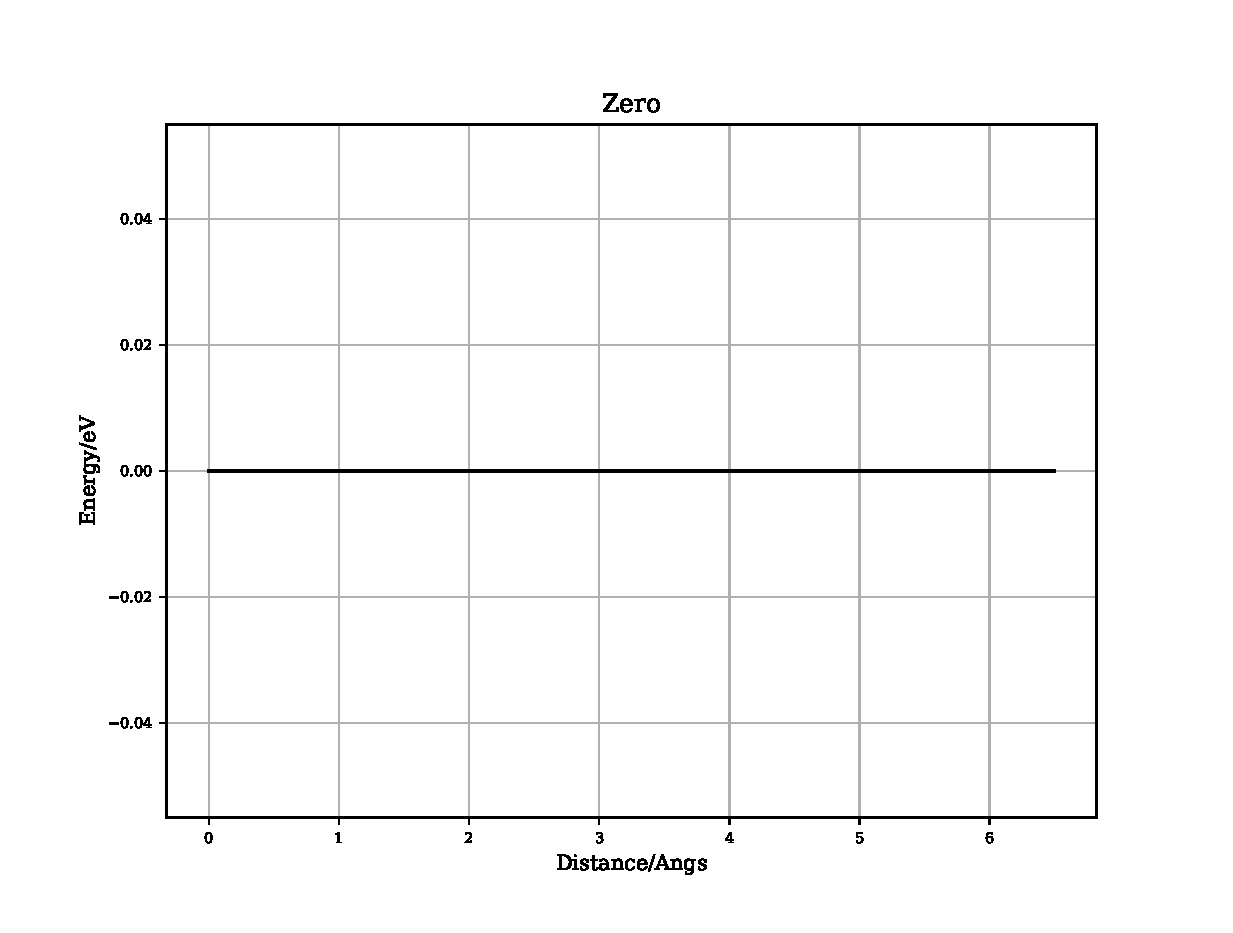
\includegraphics[scale=0.5]{appendix/functions/plots/zero.eps}
    \caption{Zero}
    \label{graph:graph1}
  \end{center}
\end{figure}
\FloatBarrier


